\documentclass[10pt,a4paper]{report}
\usepackage[utf8]{inputenc}
\usepackage{amsmath}
\usepackage{amsfonts}
\usepackage{amssymb}
\usepackage{float}
\usepackage{graphicx}
\graphicspath{{./images/}}
\usepackage{mathtools}
\DeclarePairedDelimiter\abs{\lvert}{\rvert}
\usepackage[left=3.00cm, right=3.00cm, top=3.00cm, bottom=3.00cm]{geometry}
\author{Del Prete Giovanni, Ghilardi Nicola, Polver Marco}
\title{BookSales UniBG: iterazione 0}
\begin{document}
	
	\maketitle
	\tableofcontents
	
	\section{Requisiti e scelte progettuali}
	\subsection{Obiettivi}
	\textit{BookSales UniBG} è un'applicazione web ideata con l'idea di favorire e migliorare i processi di compravendita di libri universitari all'interno dell'Università degli Studi di Bergamo. 
	\\
	Attualmente per la vendita di libri gli studenti utilizzano mezzi quali le bacheche distribuite nelle diverse sedi, gruppi sui social network e siti web di annunci oppure sfruttano le proprie conoscenze personali. Tutti questi mezzi risultano avere problemi di inefficacia dovuti alla scarsa visibilità dei libri messi in vendita oppure alla natura troppo "general purpose" dei servizi online utilizzati.\\
	\textit{BookSales UniBG} si propone di fornire un mezzo per la vendita di libri universitari che sia in grado di:
	\begin{enumerate}
		\item Facilitare l'inserimento di un'inserzione da parte di un venditore.
		\item Mostrare ai potenziali acquirenti tutti quei libri che con maggior probabilità potrebbero far parte dei loro interessi.
		\item Favorire compravendite soddisfacenti.
		\item Impedire la compravendita di appunti o libri fotocopiati.
		\item Garantire l'accesso al servizio da qualsiasi dispositivo connesso in rete.
	\end{enumerate}

	\subsection{Codice etico}
	Gli studenti che si registrano al servizio accettano di rispettare le seguenti regole:
	\begin{enumerate}
		\item E' vietato pubblicare contenuti offensivi o che possono ledere la sensibilità degli altri utenti.
		\item E' vietato cedere libri fotocopiati o scannerizzati, anche a titolo gratuito.
		\item E' vietato cedere appunti richiedendo un compenso. Gli appunti possono essere ceduti esclusivamente a titolo gratuito inserendoli nell'inserzione relativa ad un libro. Non è pertanto possibile cedere i soli appunti. 
	\end{enumerate}
	Una violazione dei precedenti punti può essere segnalata da qualsiasi utente. In particolare, per quanto riguarda il terzo punto, è possibile anche segnalare inserzioni in cui si sospetta che il venditore abbia aumentato il prezzo di un libro per includere implicitamente un pagamento di appunti ceduti insieme allo stesso.

	\subsection{Requisiti funzionali}
	Per la comprensione dei requisiti è necessario chiarire il significato dato ai seguenti termini:
	\begin{itemize}
		\item \textit{Libro}: si intende uno specifico libro in vendita, con relativa inserzione.
		\item \textit{Titolo}: si intende un elaborato generico, non una sua realizzazione fisica.
	\end{itemize}
	Esempio: "Fondamenti di meccanica per l'ingegneria" è un titolo, mentre per libro si potrebbe intendere una sua qualsiasi realizzazione fisica messa in vendita da un utente. \\
	E' inoltre necessario introdurre la classificazione degli utenti del servizio:
	\begin{itemize}
		\item Studente: si tratta di uno studente iscritto presso l'Università degli Studi di Bergamo che intende usufruire del servizio. All'interno del documento verrà anche chiamato \textit{utente}.
		\item Amministratore: si tratta di un soggetto che amministra il sito web e che potrebbe essere esterno all'università.
	\end{itemize}
	Questa classificazione risulta necessaria per comprendere i requisiti elencati in seguito, i quali possono riferirsi a classi d'utenti diverse:\\
	
	\begin{tabular}{cp{3cm}p{9cm}p{1cm}}
		Codice requisito&Nome&Descrizione\\ \hline
		AC1&Registrazione nuovo studente&Registrazione e verifica dei dati di un nuovo studente che intende usufruire del servizio. I dati da fornire obbligatoriamente durante la registrazione dovranno essere i seguenti:
		\begin{itemize}
			\item Username desiderato
			\item Nome e cognome
			\item Mail universitaria UniBG
			\item Corso di laurea e anno di corso
		\end{itemize}
		Deve essere inoltre possibile fornire dati facoltativi quali:
		\begin{itemize}
			\item Numero di telefono
			\item Mail personale (diversa da quella universitaria)
			\item Pagina Facebook
			\item Foto profilo
		\end{itemize}
		A richiesta di registrazione effettuata, il sistema deve verificare che nessuno studente si sia già registrato con l'indirizzo email universitario e lo username inseriti ed inviare all'indirizzo email fornito una email contenente una password generata casualmente e che dovrà essere utilizzata dallo studente per confermare la propria registrazione entro 3 giorni, oltre ai quali la sua registrazione verrà annullata.\\ \hline
		AC2&Accesso studente&Accesso al servizio da parte di uno studente precedentemente registrato tramite inserimento di username e password.\\ \hline
		AC3&Registrazione nuovo amministratore&Registrazione di un nuovo amministratore da parte di un soggetto che ricopre già tale ruolo. Per l'aggiunta di un amministratore sarà necessario fornire i seguenti dati necessari:
		\begin{itemize}
			\item Nome e cognome
			\item Mail personale
		\end{itemize}
		Il sistema dovrà verificare che nessun amministratore sia già stato registrato con lo stesso indirizzo email, genererà automaticamente uno username ("admin\_N", dove N è un numero naturale), una password e invierà questi dati all'indirizzo email inserito. A differenza di quanto deciso riguardo agli studenti, non sarà necessario effettuare un accesso entro 3 giorni per confermare la richiesta.\\ \hline
		AC4&Accesso amministratore&Accesso al servizio da parte di un amministratore tramite inserimento di username e password. Tale accesso dovrà essere effettuato in un'area del sito web diversa da quella preposta all'accesso degli studenti e dovrà risultare meno visibile rispetto a ques'ultima, per esempio tramite un link presente nel footer della pagina.\\ \hline
	\end{tabular}

	\begin{tabular}{cp{3cm}p{9cm}p{1cm}}
		Codice requisito&Nome&Descrizione\\ \hline
		RI1&Ricerca libro&Ricerca da parte di uno studente di un libro di testo in vendita con filtraggio basato su:
		\begin{itemize}
			\item Titolo
			\item ISBN
			\item Prezzo
			\item Voto medio del venditore
			\item Condizioni del libro:
			\begin{itemize}
				\item Classe A: libro intatto senza sottolineature o appunti.
				\item Classe B: libro intatto con sottolineature e appunti.
				\item Classe C: libro con piccoli segni d'usura, sottolineature e appunti.
				\item Classe D: libro con pagine stropicciate o rovinate, pieghe della copertina, sottolineature e appunti.
			\end{itemize}
			
		\end{itemize}\\ \hline
		RI2&Visualizzazione libri consigliati nella homepage&Visualizzazione nella homepage a seguito di un avvenuto accesso da parte di uno studente di libri potenzialmente interessanti sulla base di:
		\begin{itemize}
			\item Interesse mostrato esplicitamente dallo studente tramite inserimento di uno specifico libro nella lista "Wishlist" (\textit{RI3}) o tramite inserimento di un titolo nella lista "Titoli d'interesse" (\textit{RI4}).
			\item Ricerche effettuate dallo studente nell'ultima settimana.
			\item Interesse mostrato da studenti aventi caratteristiche simili (si considerino corso di laurea, ricerche effettuate, wishlist, titoli di interesse). Deve essere definito un metodo per la scelta delle inserzioni da visualizzare.
		\end{itemize}\\ \hline
		RI3&Inserimento libro in lista "Wishlist"&Inserimento da parte di uno studente di uno specifico libro in vendita (non un titolo) nella lista "Wishlist", la quale contiene riferimenti agli annunci che lo studente intende seguire.\\ \hline
		RI4&Inserimento titolo in lista "Titoli d'interesse"&Inserimento da parte di uno studente di un titolo nella lista "Titoli d'interesse", la quale permette allo studente di seguire facilmente tutti gli annunci relativi a libri legati a determinati titoli.\\ \hline
	\end{tabular}

	\begin{tabular}{cp{3cm}p{9cm}p{1cm}}
		Codice requisito&Nome&Descrizione\\ \hline
		I1&Inserimento annuncio&Inserimento da parte di uno studente di un annuncio per la vendita di un libro. L'inserzione deve contenere le seguenti informazioni mandatorie:
		\begin{enumerate}
			\item Titolo: deve essere selezionato da una lista di titoli già presenti nel sistema. In caso di assenza si richiede allo studente di inserire le informazioni del libro nel sistema affinché queste siano disponibili in futuro (\textit{I2}).
			\item Autore: aggiunto automaticamente tramite selezione del titolo.
			\item ISBN.
			\item Almeno una foto.
			\item Prezzo.
			\item Descrizione.	
			\item Condizioni del libro seguendo le indicazioni formalizzate in (\textit{R1}).
		\end{enumerate}
		Una volta confermata da parte dell'utente la richiesta di inserimento dell'inserzione, il sistema verifica che siano rispettate le seguenti condizioni:
		\begin{itemize}
			\item Lo studente non deve aver proposto un'inserzione relativa allo stesso libro negli ultimi 7 giorni.
			\item Il commento al libro non deve contenere parole scurrili.
		\end{itemize}
		Se l'annuncio rispetta le condizioni di cui sopra, il sistema lo inserisce nel database e conferma l'accettazione della richiesta allo studente. In caso di rifiuto dell'annuncio, il sistema richiederà allo studente di attendere in caso di mancato rispetto del primo punto p di modificare la descrizione in caso di mancato rispetto del secondo punto.\\ \hline
		I2&Modifica annuncio&Modifica del contenuto di un annuncio da parte dello studente a cui appartiene.\\ \hline
	\end{tabular}
	\newpage
	\begin{tabular}{cp{3cm}p{9cm}p{1cm}}
		Codice requisito&Nome&Descrizione\\ \hline
		I3&Inserimento di un nuovo titolo&Inserimento da parte di uno studente di un titolo assente dal sistema. Le informazioni da fornire sono le seguenti:
		\begin{itemize}
			\item Titolo
			\item Autore/i
			\item ISBN
			\item Categoria (informatica, meccanica, letteratura latina, economia aziendale, ...)
		\end{itemize}
		Il sistema verifica che nessun altro titolo con il medesimo ISBN sia stato inserito in precedenza e, se ciò non è avvenuto, inserisce il titolo nel database e crea automaticamente una pagina del titolo contenente le informazioni fornite.\\ \hline
		U1&Ricerca studente&Ricerca di studenti da parte di un utente con filtraggio basato su:
		\begin{itemize}
			\item Username
			\item Nome e cognome
			\item Corso di laurea
			\item Anno di corso
		\end{itemize}\\ \hline
		U2&Accesso pagina studente&Accesso alla pagina personale di un altro studente, la quale deve contenere informazioni quali:
		\begin{itemize}
			\item Contatti (numero di telefono, mail, pagina Facebook, ...)
			\item Numero di libri venduti
			\item Numero di libri acquistati
			\item Voto medio recensioni ricevute
			\item Numero di recensioni effettuate (sia nel ruolo di venditore che in quello di acquirente)
			\item Recensioni ricevute in qualità di venditore
			\item Recensioni ricevute in qualità di acquirente
			\item Libri in vendita
		\end{itemize}\\ \hline
		U2.1&Accesso pagina personale studente&Accesso alla propria pagina personale da parte di uno studente. La pagina deve fornire le medesime informazioni fornite in \textit{U2}, ma deve risultare sempre accessibile con un solo click, qualunque sia la pagina del sito web aperta nell'istante corrente.\\ \hline
		U3&Modifica informazioni personali studente&Modifica da parte di uno studente delle informazioni mostrate nella propria pagina personale.\\ \hline
	\end{tabular}
	\newpage
	
	\begin{tabular}{cp{3cm}p{9cm}p{1cm}}
		Codice requisito&Nome&Descrizione\\ \hline
		U4&Accesso pagina personale amministratore&Accesso alla propria pagina personale da parte di un amministratore. La pagina personale di un amministratore deve mostrare le seguenti informazioni:
		\begin{itemize}
			\item Username.
			\item Nome e cognome.
			\item Numero di segnalazioni gestite.
			\item Numero di richieste d'assistenza gestite.
		\end{itemize}\\ \hline
		T1&Ricerca pagina titolo&Ricerca da parte dell'utente della pagina relativa ad un titolo. La pagina deve contenere, se presenti, informazioni riguardanti gli argomenti trattati dal libro e le recensioni degli utenti sull'utilità del libro ai fini dell'esame.\\ \hline
		T2&Modifica pagina titolo&Modifica della pagina contenente le informazioni di un titolo da parte di un utente. Le informazioni che possono essere aggiunte sono le seguenti:
		\begin{itemize}
			\item Immagine della copertina
			\item Argomenti trattati
		\end{itemize}\\ \hline
		V1&Vendita libro&Comunicazione da parte del venditore dell'avvenuta cessione del libro legato ad una specifica inserzione. Il venditore deve fornire come informazione il nome utente dell'acquirente. Una volta avvenuto questo, il sistema deve inviare una email all'acquirente in cui viene chiesto di confermare l'acquisto del libro (\textit{V2}).\\ \hline
		V2&Richiesta conferma acquisto&Il sistema invia all'utente citato dal venditore come acquirente una email per richiedere la conferma dell'acquisto. L'email deve contenere un link ad una pagina in cui l'acquirente potrà confermare o negare l'acquisto (\textit{V3}).\\ \hline
		V3&Conferma acquisto&Conferma o negazione dell'acquisto di un libro da parte dell'utente che è stato indicato dal venditore quale l'acquirente del libro oggetto della cessione. La pagina deve contenere un riassunto dell'inserzione in questione (foto principale, titolo, nome utente del venditore e prime 5 righe della descrizione).
		In caso di conferma dell'acquisto:
		\begin{itemize}
			\item l'acquirente verrà invitato a recensire il venditore;
			\item il libro verrà rimosso dall'elenco dei libri in vendita e da tutte le liste personali ("wishlist" e "titoli d'interesse") in cui è presente;
			\item verranno aggiornati i dati relativi al numero di libri venduti e acquistati dei due utenti coinvolti;
			\item il sistema invierà una email al venditore per comunicargli l'avvenuta conferma dell'acquisto ed invitarlo a recensire l'acquirente.
		\end{itemize}
		In caso di negazione dell'acquisto, il venditore deve essere notificato via email dell'avvenuto ed invitato a rieffettuare la procedura \textit{V1} selezionando un utente differente. \\ \hline
	\end{tabular}

	\begin{tabular}{cp{3cm}p{9cm}p{1cm}}
		Codice requisito&Nome&Descrizione\\ \hline
		RE1&Recensione venditore&Inserimento da parte di un utente acquirente di una recensione del venditore di uno specifico libro. Questo dovrà risultare possibile soltanto dopo la conferma dell'acquisto di un libro. La recensione dovrà contenere un valore intero compreso tra 0 e 5 (indicato tramite stelle) ed un commento.\\ \hline
		RE2&Recensione acquirente&Inserimento da parte di un utente venditore di una recensione dell'acquirente di uno specifico libro. Questo dovrà risultare possibile soltanto dopo la conferma dell'acquisto di un libro. La recensione dovrà contenere un valore intero compreso tra 0 e 5 (indicato tramite stelle) ed un commento.\\ \hline
		RE3&Recensione titolo&Inserimento da parte di un utente qualsiasi di una recensione di un qualsiasi titolo. La recensione dovrà contenere un valore intero compreso tra 0 e 5 (indicato tramite stelle) ed un commento.\\ \hline
	\end{tabular}

	
	\section{Casi d'uso}
	Di seguito sono riportati i diagrammi dei casi d'uso relativo ad amministratori, studenti ed utenti generici.
	
	\begin{figure}[H]
		\centering
		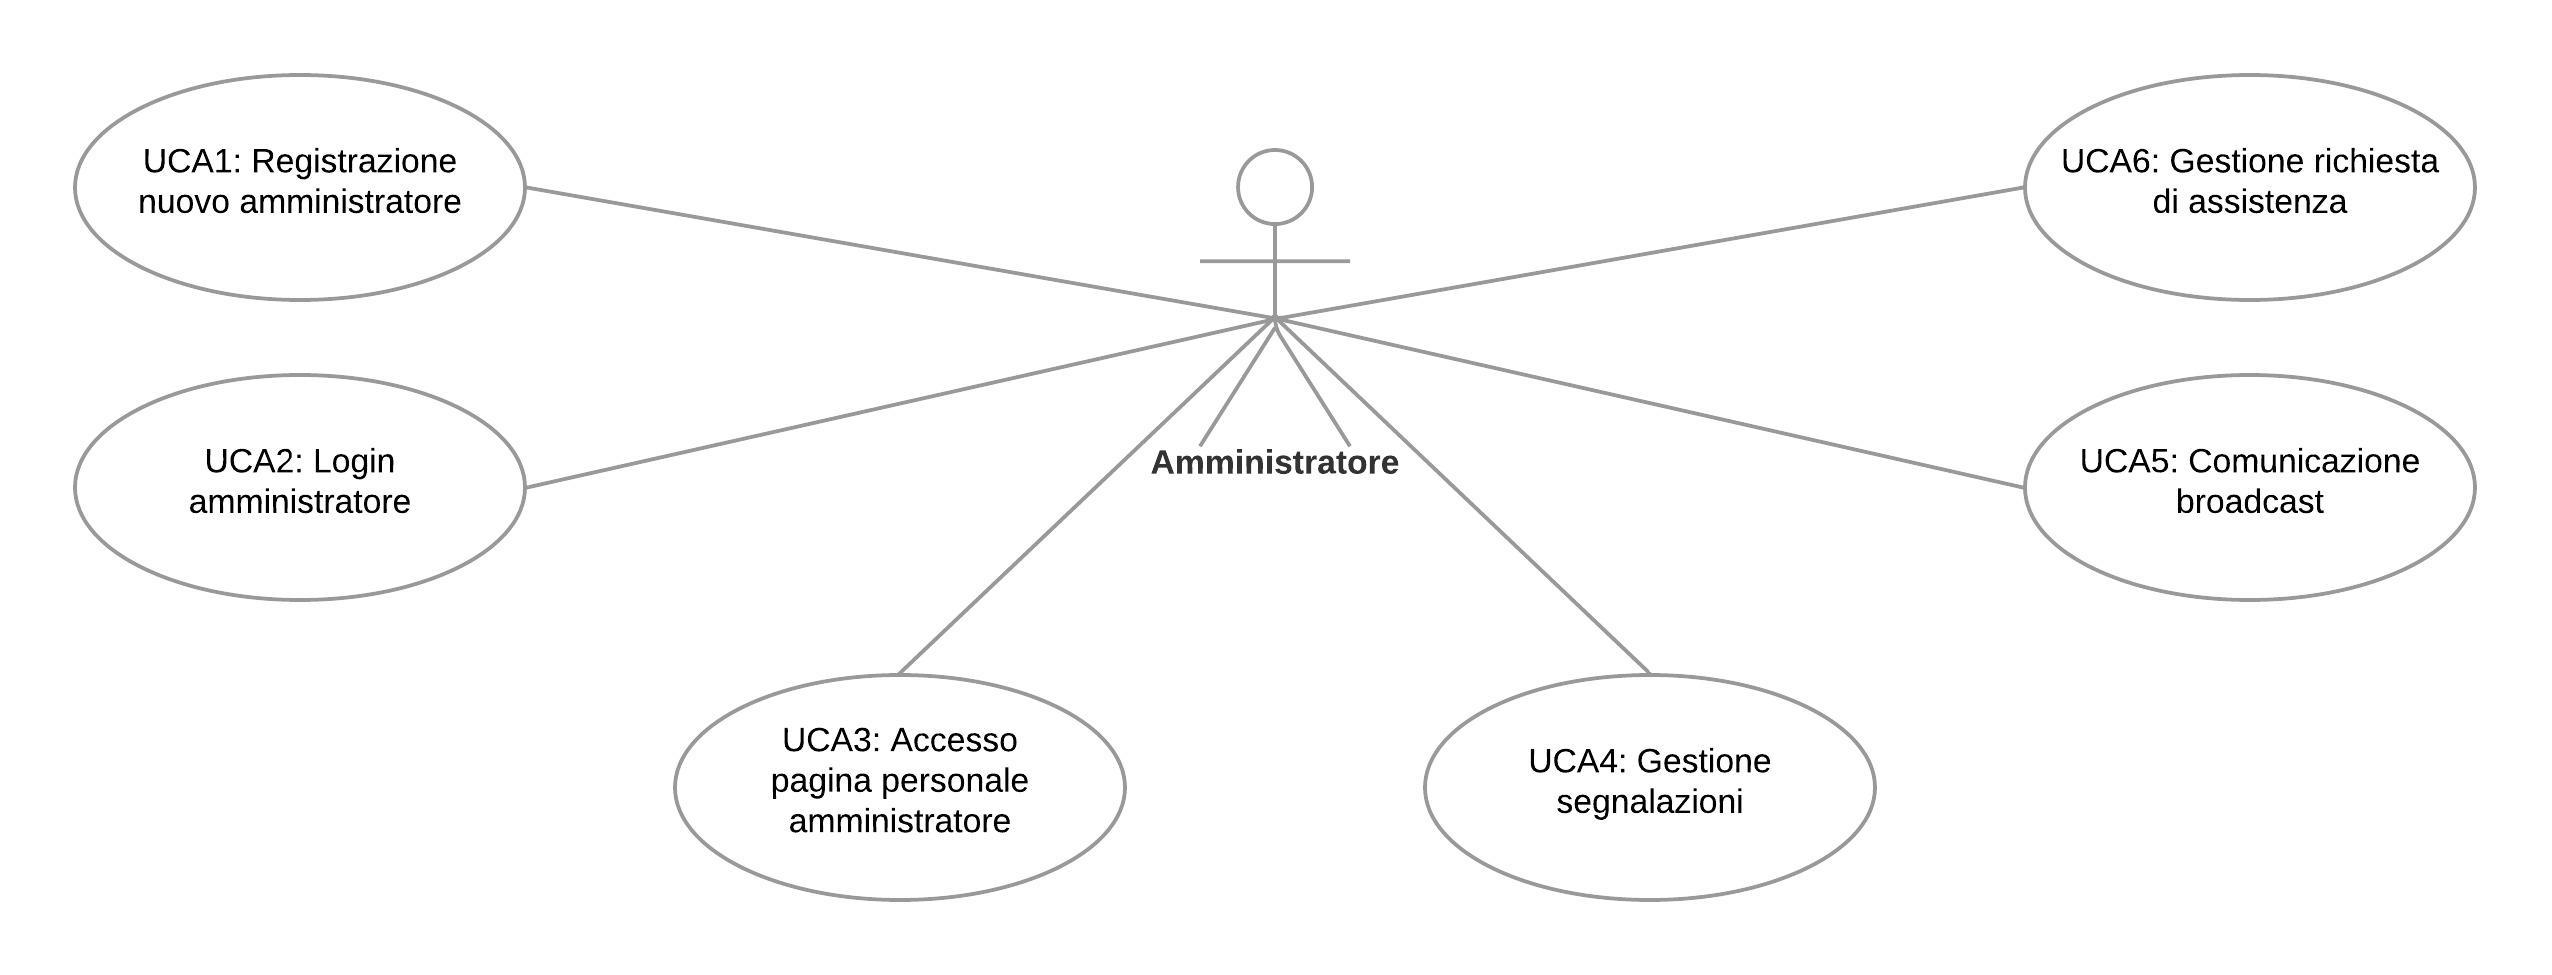
\includegraphics[height=12cm, width=17cm, keepaspectratio]{gua_uc}
		\caption{Casi d'uso per utente generico e amministratore}
	\end{figure}

	\begin{figure}[H]
		\centering
		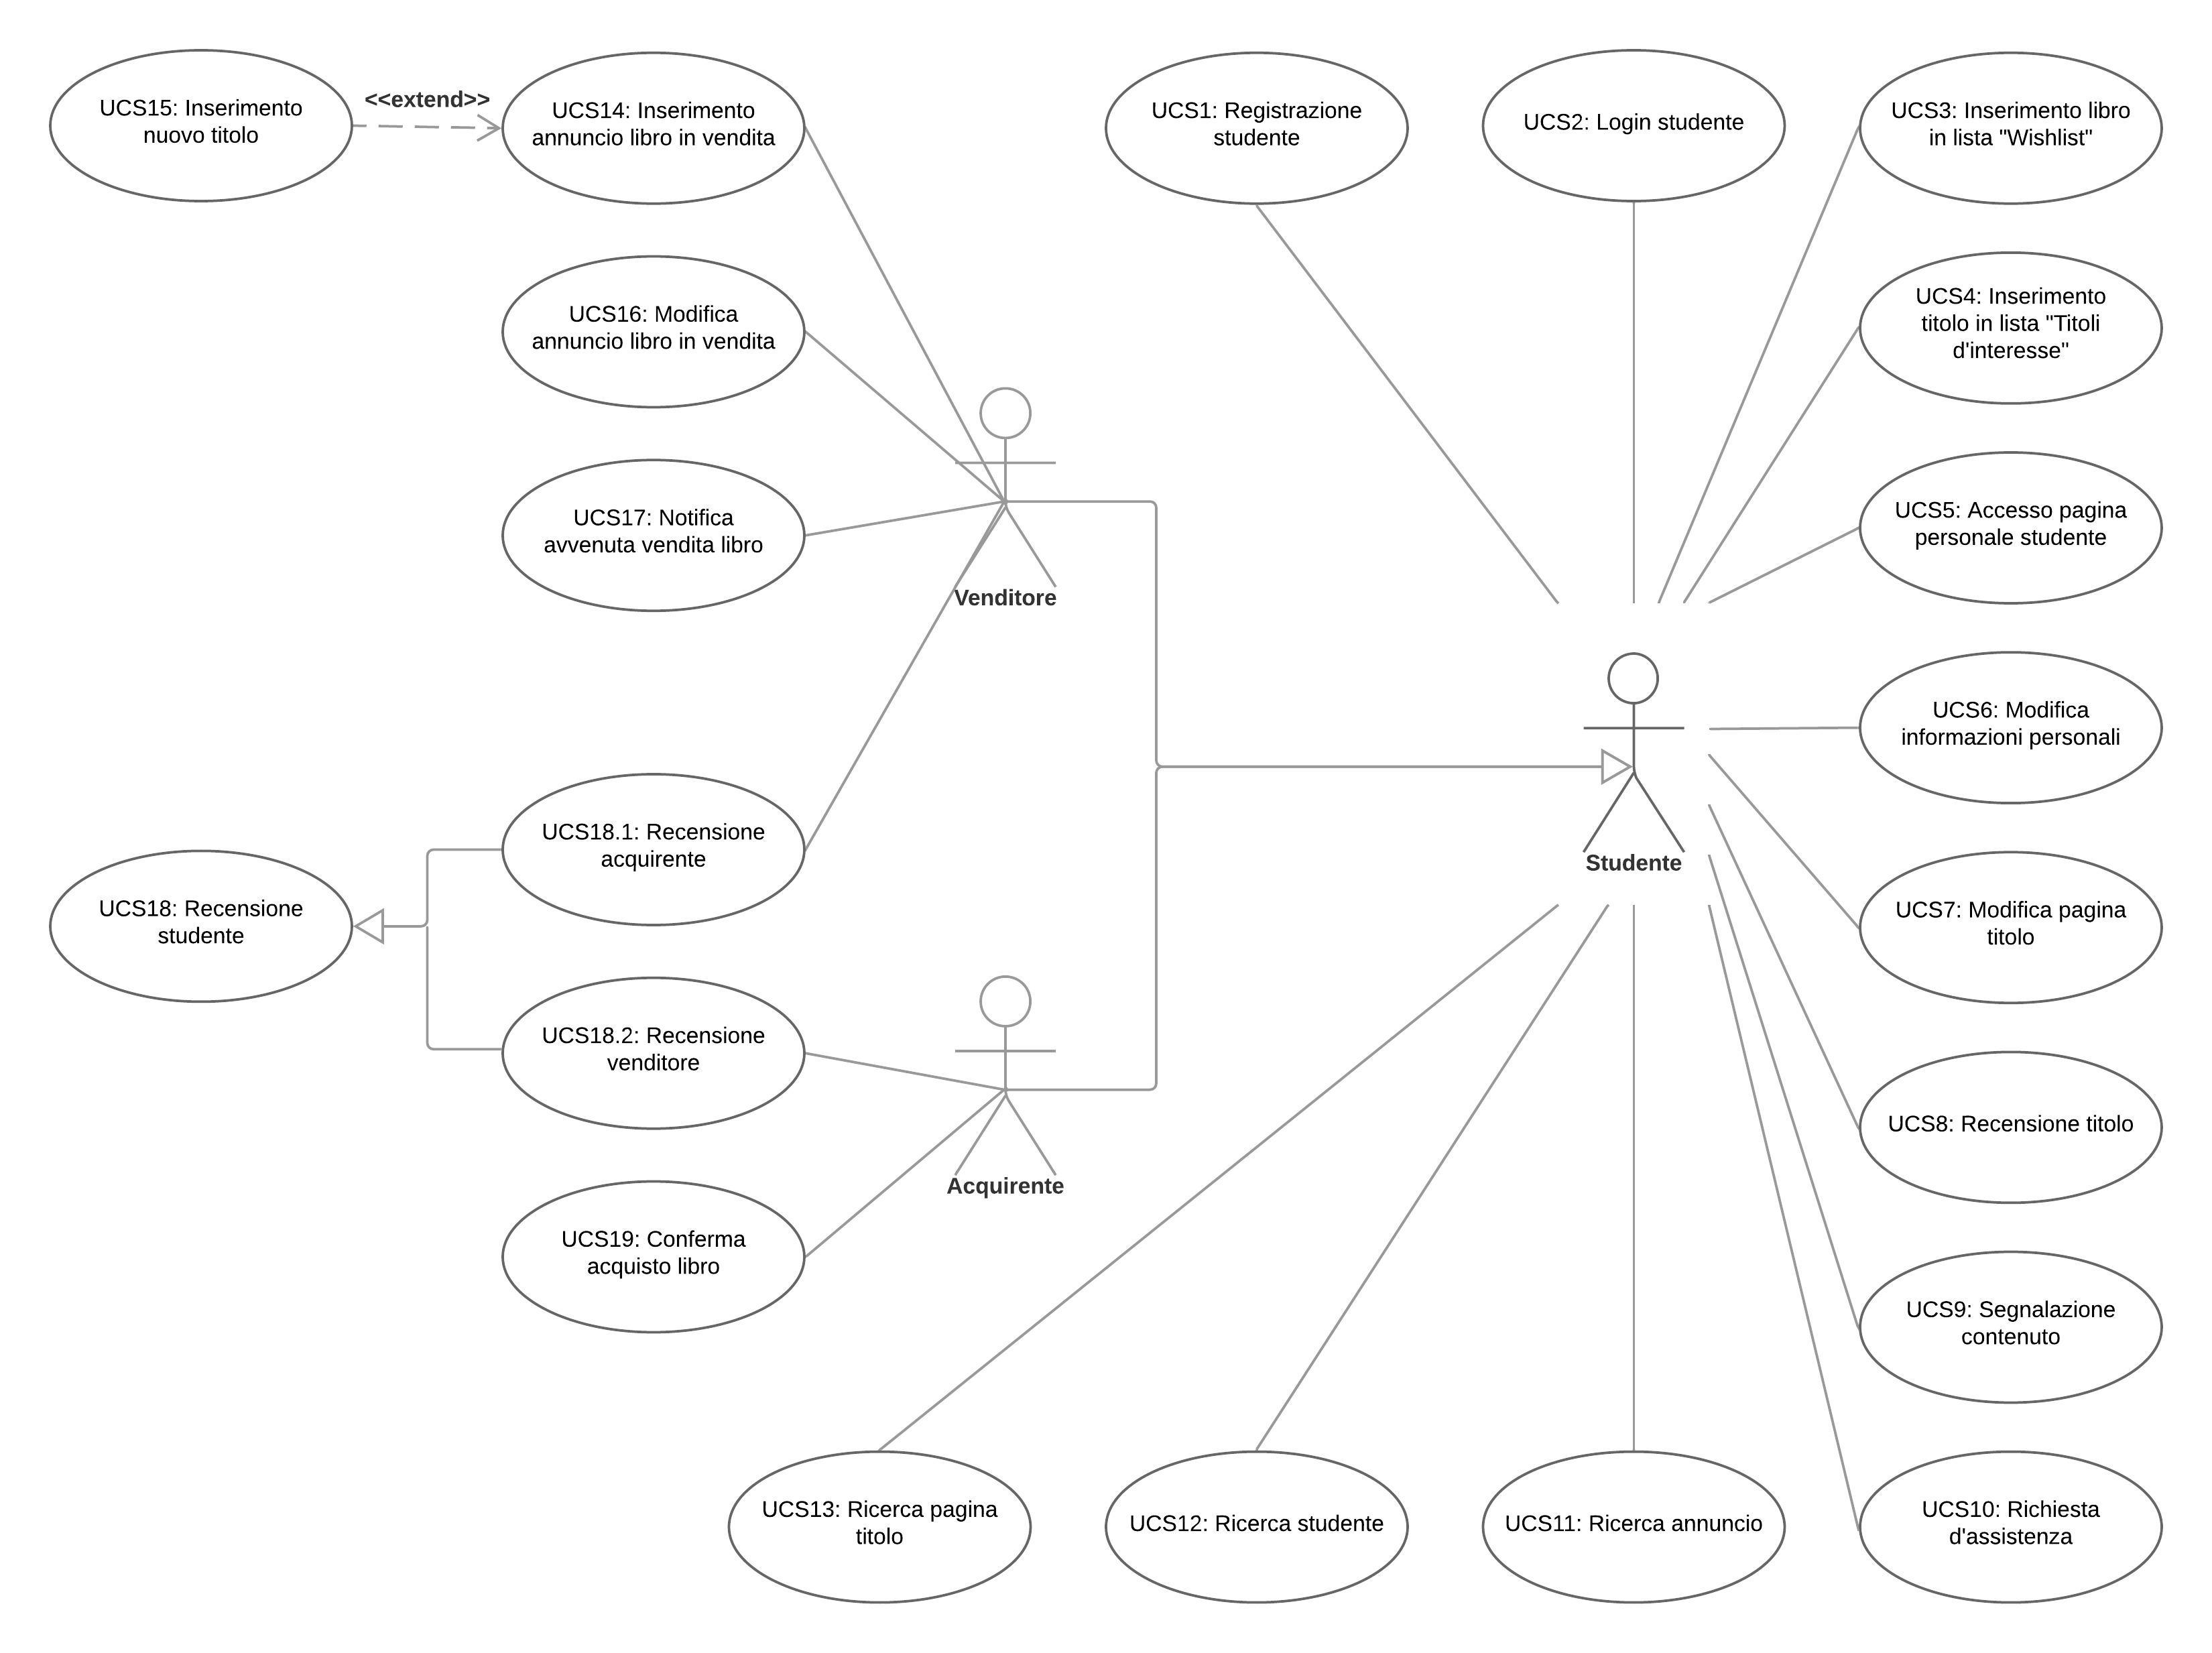
\includegraphics[height=19cm, width=17cm, keepaspectratio]{st_uc}
		\caption{Casi d'uso per studente}
	\end{figure}

	\subsection{UCA1: Registrazione nuovo amministratore}
	\begin{tabular}{lp{0.8\textwidth}}
		\textbf{Descrizione}&Un amministratore effettua la registrazione di un nuovo amministratore del servizio.\\
		\\
		\textbf{Requisiti coperti}&AC3\\
		\\
		\textbf{Attori coinvolti}&Amministratore\\
		\\
		\textbf{Precondizioni}&\begin{itemize}
			\item L'amministratore che effettua la registrazione di un secondo amministratore ha affettuato il login.
			\item L'amministratore che deve essere registrato è assente dal database del sistema.
		\end{itemize}\\
		\\
		\textbf{Postcondizioni}&I dati relativi al nuovo amministratore vengono salvati nel database.\\
		\\
		\textbf{Processo}&Di seguito è descritto il processo:
		\begin{enumerate}
			\item L'amministratore che si occupa della registrazione di un collega accede alla pagina relativa alla registrazione di un nuovo amministratore.
			\item Il sistema mostra una serie di campi che devono essere compilati per la registrazione di un amministratore:
			\begin{itemize}
				\item Nome e cognome.
				\item Indirizzo email personale.
			\end{itemize}
			\item L'amministratore compila i campi ed esegue il comando di registrazione.
			\item Il sistema verifica che i campi siano stati compilati correttamente:
			\begin{itemize}
				\item Entrambi i campi devono essere compilati.
				\item L'indirizzo email deve essere formattato correttamente (nome@dominioprivato.dominio\_primo\_livello).
			\end{itemize}
			\item Sulla base del risultato della verifica il sistema si comporta in modo diverso:
			\begin{itemize}
				\item Se i campi sono stati compilati in modo sintatticamente corretto, il sistema continua con il successivo passo della registrazione.
				\item Se i campi non sono stati compilati in modo sintatticamente corretto, il sistema non esegue la registrazione e mostra un riquadro rosso con la scritta "Campi compilati in modo errato".
			\end{itemize}
			\item Il sistema verifica che nessun amministratore con il medesimo indirizzo email sia già presente nel database.
		\end{enumerate}
	\end{tabular}

	\begin{tabular}{lp{0.8\textwidth}}
		\textbf{Processo}&\begin{enumerate}
			\setcounter{enumi}{6}
			\item In base al risultato della ricerca precedente il sistema si può comportare in due modi:
			\begin{itemize}
				\item Se l'indirizzo email è già stato utilizzato da un altro amministratore, il sistema mostra un riquadro rosso con la scritta "Indirizzo email già utilizzato" e non effettua la registrazione.
				\item Se l'indirizzo email non è stato utilizzato da alcun amministratore, i dati relativi al nuovo amministratore vengono inseriti nel database insieme ad una password da 10 caratteri generata automaticamente dal sistema (deve includere lettere, numeri e simboli speciali) e uno username anch'esso generato automaticamente e che abbia la struttura "admin\_N", dove N corrisponde al numero totale di amministratori del sistema in seguito alla registrazione del nuovo amministratore.
			\end{itemize}
			\item Se la registrazione è avvenuta con successo, il sistema invia all'indirizzo del nuovo amministratore una mail contenente il nome utente e la password che dovrà utilizzare per effettuare l'accesso.
		\end{enumerate}
	\end{tabular}
	
	\subsection{UCA2: Login amministratore}
	\begin{tabular}{lp{0.8\textwidth}}
		\textbf{Descrizione}&Un amministratore effettua il login al sistema.\\
		\\
		\textbf{Requisiti coperti}&AC4\\
		\\
		\textbf{Attori coinvolti}&Amministratore\\
		\\
		\textbf{Precondizioni}&L'amministratore è presente nel database del sistema.\\
		\\
		\textbf{Postcondizioni}&L'amministratore può svolgere tutte le attività consentite al suo ruolo e ad un utente generico.\\
		\\
		\textbf{Processo}&Di seguito è descritto il processo:
		\begin{enumerate}
			\item L'amministratore accede alla pagina per il login dedicata agli amministratori del sistema.
			\item Il sistema visualizza due campi in cui inserire indirizzo email e password.
			\item L'amministratore inserisce indirizzo email e password e richiede l'accesso.
			\item Il sistema verifica che esista un amministratore registrato con l'indirizzo email inserito e in caso affermativo verifica che la password inserita sia corretta.
			\item In base al risultato della ricerca precedente il sistema si può comportare in due modi:
			\begin{itemize}
				\item Se nessun amministratore risulta registrato con tale username o la password è errata, il sistema mostra un riquadro rosso con la scritta "Dati d'accesso errati" ed impedisce l'accesso.
				\item Se i dati inseriti sono corretti, il sistema permette l'accesso all'amministratore ed apre la pagina personale dello stesso.
			\end{itemize}
		\end{enumerate}
	\end{tabular}
	
	\subsection{UCA3: Accesso pagina personale amministratore}
	\begin{tabular}{lp{0.8\textwidth}}
		\textbf{Descrizione}&Un amministratore vuole accedere alla propria pagina personale.\\
		\\
		\textbf{Requisiti coperti}&U4\\
		\\
		\textbf{Attori coinvolti}&Amministratore\\
		\\
		\textbf{Precondizioni}&L'amministratore ha effettuato l'accesso.\\
		\\
		\textbf{Postcondizioni}&Il sistema mostra la pagina contenente le informazioni personali e i dati legati all'attività dell'amministratore.\\
		\\
		\textbf{Processo}&Di seguito è descritto il processo:
		\begin{enumerate}
			\item L'amministratore accede alla propria pagina personale.
			\item Il sistema mostra le seguenti informazioni riguardanti l'amministratore:
			\begin{itemize}
				\item Username.
				\item Nome e cognome.
				\item Numero di segnalazioni gestite.
				\item Numero di richieste d'assistenza gestite.
				\item Data d'iscrizione al servizio.
			\end{itemize}
		\end{enumerate}
	\end{tabular}
	
	
	\subsection{UCS1: Registrazione studente}
	\begin{tabular}{lp{0.8\textwidth}}
		\textbf{Descrizione}&Uno studente si registra al servizio.\\
		\\
		\textbf{Requisiti coperti}&AC1\\
		\\
		\textbf{Attori coinvolti}&Studente\\
		\\
		\textbf{Precondizioni}&Lo studente che effettua la registrazione è assente dal database del sistema.\\
		\\
		\textbf{Postcondizioni}&I dati relativi al nuovo studente vengono salvati nel database.\\
		\\
		\textbf{Processo}&Di seguito è descritto il processo:
		\begin{enumerate}
			\item Lo studente accede alla pagina per la registrazione.
			\item Il sistema mostra una serie di campi da compilare:
			\begin{itemize}
				\item \textit{Campi obbligatori}:
				\begin{itemize}
					\item Username desiderato
					\item Nome e cognome
					\item Mail universitaria UniBG
					\item Corso di laurea e anno di corso
				\end{itemize}
				\item \textit{Campi facoltativi}:
				\begin{itemize}
					\item Numero di telefono personale
					\item Mail personale
					\item Link alla propria pagina Facebook
					\item Foto profilo
				\end{itemize}
			\end{itemize}
			\item Lo studente compila i campi erichiede la registrazione al servizio.
			\item Il sistema verifica che tutti i campi obbligatori siano stati compilati e che rispettino le seguenti condizioni:
			\begin{itemize}
				\item Lo username non deve essere già stato utilizzato da un altro utente e non deve contenere la parola "admin".
				\item La mail universitaria inserita deve terminare con uno tra i suffissi "@studenti.unibg.it" e "@unibg.it" e non deve essere già stata utilizzata.
			\end{itemize}
		\end{enumerate}
	\end{tabular}

	\begin{tabular}{lp{0.8\textwidth}}
		\textbf{Processo}&\begin{enumerate}
			\setcounter{enumi}{4}
			\item In base al risultato delle verifiche al punto precedente il sistema si comporta in modi diversi:
			\begin{itemize}
				\item Se non tutti i campi obbligatori sono stati compilati, il sistema non effettua la registrazione e mostra un riquadro rosso con la scritta "Tutti i campi obbligatori devono essere compilati".
				\item Se lo username scelto risulta già utilizzato o contiene la parola "admin", il sistema non effettua la registrazione e mostra un riquadro rosso con la scritta "Username non disponibile".
				\item Se la mail utilizzata non rispetta le regole di cui sopra, il sistema non effettua la registrazione e mostra un riquadro rosso con la scritta "L'indirizzo email deve appartenere al dominio unibg.it".
				\item Se la mail inserita risulta essere già presente nel database, il sistema non effettua la registrazione e mostra un riquadro giallo con la scritta "Indirizzo email già presente nel sistema, effettua il login".
				\item Se tutte le condizioni sono rispettate, il sistema esegue le seguenti operazioni:
				\begin{enumerate}
					\item Inserimento nel database dei dati dell'utente e della data di registrazione.
					\item Generazione automatica di una password da 10 caratteri contenente numeri, lettere e simboli speciali.
					\item Inserimento della password generata al passo precedente nel database.
					\item Invio di una mail contenente i dati d'accesso all'indirizzo universitario inserito dallo studente.
				\end{enumerate}
			\end{itemize}
			\item Lo studente ha 3 giorni di tempo per effettuare il primo accesso al servizio:
			\begin{itemize}
				\item Se il primo accesso avviene entro il termine stabilito, il sistema setta i dati dello studente come confermati.
				\item Se il termine scade senza che il primo accesso sia stato effettuato, il sistema elimina i dati dello studente dal sistema.
			\end{itemize}
		\end{enumerate}
	\end{tabular}
	
	\subsection{UCS2: Login studente}
	\begin{tabular}{lp{0.8\textwidth}}
		\textbf{Descrizione}&Uno studente effettua il login al sistema.\\
		\\
		\textbf{Requisiti coperti}&AC2, RI2\\
		\\
		\textbf{Attori coinvolti}&Studente\\
		\\
		\textbf{Precondizioni}&Lo studente è presente nel database del sistema.\\
		\\
		\textbf{Postcondizioni}&Lo studente può svolgere tutte le attività consentite al suo ruolo e ad un utente generico.\\
		\\
		\textbf{Processo}&Di seguito è descritto il processo:
		\begin{enumerate}
			\item Lo studente accede alla pagina per il login dedicata agli studenti.
			\item Il sistema visualizza due campi in cui inserire username e password.
			\item Lo studente inserisce username e password e richiede l'accesso.
			\item Il sistema verifica che esista uno studente registrato con lo username inserito e in caso affermativo verifica che la password inserita sia corretta.
			\item In base al risultato della ricerca precedente il sistema si può comportare in due modi:
			\begin{itemize}
				\item Se nessuno studente risulta registrato con tale username o la password è errata, il sistema mostra un riquadro rosso con la scritta "Username e/o password errati" ed impedisce l'accesso.
				\item Se i dati inseriti sono corretti, il sistema permette l'accesso allo studente e verifica se lo studente è sospeso dal servizio per numero eccessivo di segnalazioni ricevute:
				\begin{itemize}
					\item Se lo studente risulta sospeso, gli viene permessa la sola visualizzazione di una pagina che lo informa del suo status.
					\item Se lo studente non risulta sospeso, viene aperta la homepage del sito, la quale sulla base dei dati relativi allo specifico studente deve mostrare i seguenti contenuti:
					\begin{itemize}
						\item Annunci presenti nella "wishlist" di studenti simili (per corso di laurea, anno di corso, ricerche effettuate, wishlist e titoli d'interesse).
						\item Annunci presenti nella "wishlist" o legati a titoli presenti nella lista "Titoli d'interesse" dello studente.
					\end{itemize}
				\end{itemize}
			\end{itemize} 
		\end{enumerate}
	\end{tabular}

	\subsection{UCS3: Inserimento libro in lista "Wishlist"}
	\begin{tabular}{lp{0.8\textwidth}}
		\textbf{Descrizione}&Uno studente inserisce un libro in vendita nella propria lista "Wishlist".\\
		\\
		\textbf{Requisiti coperti}&RI3\\
		\\
		\textbf{Attori coinvolti}&Studente\\
		\\
		\textbf{Precondizioni}&Lo studente ha effettuato il login ed ha aperto la pagina relativa ad un annuncio.\\
		\\
		\textbf{Postcondizioni}&Il libro fa parte della "Wishlist" dello studente.\\
		\\
		\textbf{Processo}&Di seguito è descritto il processo:
		\begin{enumerate}
			\item Lo studente richiede l'inserimento del libro nella propria "Wishlist".
			\item Il sistema inserisce il libro nella "Wishlist" dello studente e mostra un riquadro verde con la scritta "Libro inserito nella tua Wishlist".
		\end{enumerate}
	\end{tabular}

	\subsection{UCS4: Inserimento titolo in lista "Titoli d'interesse"}
	\begin{tabular}{lp{0.8\textwidth}}
		\textbf{Descrizione}&Uno studente inserisce un titolo nella propria lista "Titoli d'interesse".\\
		\\
		\textbf{Requisiti coperti}&RI4\\
		\\
		\textbf{Attori coinvolti}&Studente\\
		\\
		\textbf{Precondizioni}&Lo studente ha effettuato il login ed ha aperto la pagina relativa ad un titolo.\\
		\\
		\textbf{Postcondizioni}&Il titolo fa parte della lista "Titoli d'interesse" dello studente.\\
		\\
		\textbf{Processo}&Di seguito è descritto il processo:
		\begin{enumerate}
			\item Lo studente richiede l'inserimento del titolo nella propria lista "Titoli d'interesse".
			\item Il sistema inserisce il libro nella lista "Titoli d'interesse" dello studente e mostra un riquadro verde con la scritta "Titolo inserito nella tua  lista 'Titoli d'interesse'".
		\end{enumerate}
	\end{tabular}

	\subsection{UCS5: Accesso pagina persinale studente}
	\begin{tabular}{lp{0.8\textwidth}}
		\textbf{Descrizione}&Uno studente vuole accedere alla propria pagina personale.\\
		\\
		\textbf{Requisiti coperti}&U2.1\\
		\\
		\textbf{Attori coinvolti}&Studente\\
		\\
		\textbf{Precondizioni}&Lo studente ha effettuato il login.\\
		\\
		\textbf{Postcondizioni}&Il sistema mostra la pagina contenente le informazioni personali e i dati legati all'attività dello studente.\\
		\\
		\textbf{Processo}&Di seguito è descritto il processo:
		\begin{enumerate}
			\item Lo studente accede alla propria pagina personale.
			\item Il sistema mostra le medesime informazioni mostrate in caso di apertura della pagina personale di un altro studente, come descritto nel caso d'uso \textit{UCG2}.
		\end{enumerate}
	\end{tabular}

	\subsection{UCS6: Modifica impostazioni personali}
	\begin{tabular}{lp{0.8\textwidth}}
		\textbf{Descrizione}&Uno studente vuole modificare le proprie informazioni personali.\\
		\\
		\textbf{Requisiti coperti}&U3\\
		\\
		\textbf{Attori coinvolti}&Studente\\
		\\
		\textbf{Precondizioni}&Lo studente ha effettuato il login ed ha aperto la propria pagina personale.\\
		\\
		\textbf{Postcondizioni}&Il sistema permette allo studente di modificare le proprie informazioni personali e salva i cambiamenti apportati nel database.\\
		\\
		\textbf{Processo}&Di seguito è descritto il processo:
		\begin{enumerate}
			\item Lo studente accede alla propria pagina personale e richiede la modifica dei propri dati personali.
			\item Il sistema mostra una pagina contenente un elenco di campi compilabili (i campi relativi ad informazioni già fornite risultano precompilati, ma comunque modificabili) dallo studente:
			\begin{itemize}
				\item Corso di laurea e anno di corso
				\item Numero di telefono personale
				\item Indirizzo email personale
				\item Link alla pagina Facebook personale
				\item Foto profilo
			\end{itemize}
			\item Lo studente può modificare tutti i campi per poi confermare le modifiche apportate.
			\item Il sistema verifica la correttezza dei dati inseriti:
			\begin{itemize}
				\item La lunghezza del numero di telefono personale, se inserito, deve essere di 10 cifre.
				\item L'indirizzo email personale, se inserito, deve contenere un simbolo '@' seguito dal nome di un dominio.
				\item Il link alla pagina Facebook personale, se inserito, deve essere un link ad una pagina appartenente a Facebook.
			\end{itemize}
			\item Sulla base del risultato delle verifiche effettuate al passo precedente, il sistema esegue operazioni differenti:
			\begin{itemize}
				\item Se i dati inseriti sono corretti, il sistema salva nel database i nuovi dati relativi allo studente.
				\item Se i dati inseriti non sono corretti, il sistema non effettua il salvataggio dei dati e mostra un riquadro rosso con la scritta "Dati incorretti".
			\end{itemize}
		\end{enumerate}
	\end{tabular}

	\subsection{UCS7: Modifica pagina titolo}
	\begin{tabular}{lp{0.8\textwidth}}
		\textbf{Descrizione}&Uno studente vuole modificare le proprie informazioni personali.\\
		\\
		\textbf{Requisiti coperti}&T2\\
		\\
		\textbf{Attori coinvolti}&Studente\\
		\\
		\textbf{Precondizioni}&Lo studente ha effettuato il login ed ha aperto la pagina relativa ad uno specifico titolo.\\
		\\
		\textbf{Postcondizioni}&Il sistema permette allo studente di modificare le informazioni contenute nella pagina di un titolo.\\
		\\
		\textbf{Processo}&Di seguito è descritto il processo:
		\begin{enumerate}
			\item Lo studente accede alla pagina relativa ad un titolo e ne richiede la modifica.
			\item Il sistema mostra una pagina contenente un elenco di campi compilabili (i campi relativi ad informazioni già fornite risultano precompilati, ma comunque modificabili) dallo studente:
			\begin{itemize}
				\item Immagine della copertina del libro.
				\item Descrizione degli argomenti trattati.
			\end{itemize}
			\item Il sistema salva le modifiche effettuate nel database e mostra un riquadro verde con la scritta "Modifica della pagina avvenuta con successo".
		\end{enumerate}
	\end{tabular}

	\subsection{UCS8: Recensione titolo}
	\begin{tabular}{lp{0.8\textwidth}}
		\textbf{Descrizione}&Uno studente vuole recensire un titolo.\\
		\\
		\textbf{Requisiti coperti}&RE3\\
		\\
		\textbf{Attori coinvolti}&Studente\\
		\\
		\textbf{Precondizioni}&Lo studente ha effettuato il login ed ha aperto la pagina relativa ad uno specifico titolo.\\
		\\
		\textbf{Postcondizioni}&Il sistema permette allo studente di recensire il titolo e mostra la recensione sulla pagina del titolo stesso.\\
		\\
		\textbf{Processo}&Di seguito è descritto il processo:
		\begin{enumerate}
			\item Lo studente accede alla pagina relativa ad un titolo e richiede di recensire il titolo stesso.
			\item Il sistema mostra una pagina contenente un elenco di campi che devono essere compilati:
			\begin{itemize}
				\item Titolo della recensione
				\item Voto: da 0 a 5 con passo di 0.5
				\item Testo della recensione
			\end{itemize}
			\item Il sistema salva le informazioni contenute nella recensione nel database e mostra la recensione sulla pagina del titolo.
		\end{enumerate}
	\end{tabular}

	
	\subsection{UCS11: Ricerca annuncio}
	\begin{tabular}{lp{0.8\textwidth}}
		\textbf{Descrizione}&Uno studente effettua la ricerca di un libro tra gli annunci pubblicati.\\
		\\
		\textbf{Requisiti coperti}&RI1\\
		\\
		\textbf{Attori coinvolti}&Studente\\
		\\
		\textbf{Precondizioni}&Lo studente ha effettuato il login.\\
		\\
		\textbf{Postcondizioni}&Vengono mostrati gli annunci compatibili con le keyword e i filtri inseriti dall'utente.\\
		\\
		\textbf{Processo}&Di seguito è descritto il processo:
		\begin{enumerate}
			\item Lo studente accede alla pagina relativa alla ricerca di annunci di libri in vendita.
			\item Il sistema mostra una pagina contenente una serie di campi (filtri) compilabili dall'utente per la ricerca degli annunci.
			\item Lo studente imposta i filtri sui risultati che intende ricevere. In particolare l'utente può usare i seguenti filtri:
			\begin{itemize}
				\item Titolo: può essere selezionato da una lista previa utilizzo del filtro precedente, oppure essere digitato manualmente dall'utente generico (non case-sensitive).
				\item ISBN.
				\item Prezzo: possono essere scelti un prezzo massimo e/o un prezzo minimo.
				\item Voto medio del venditore: possono essere scelti un voto medio minimo e/o un voto medio massimo del venditore. Questo filtro non viene applicato a quei venditori che non hanno ancora ricevuto una recensione.
				\item Condizione del libro: possono essere scelti una classe minima e/o una classe massima tra quelle introdotte nel requisito (\textit{RI1}).			
			\end{itemize}
			\item Il sistema ricerca tra gli annunci nel database i libri che risultano coerenti con i filtri imposti e mostra i risultati in ordine decrescente rispetto al voto medio del venditore. In particolare per ogni risultato verranno mostrati titolo, foto, prezzo, condizione del libro e username del venditore, mentre la descrizione del libro viene omessa.
			\item Lo studente può scegliere il fattore da utilizzare per l'ordinamento dei risultati (per tutti i fattori è possibile la visualizzazione sia in ordine crescente che decrescente):
			\begin{itemize}
				\item Voto medio del venditore.
				\item Data d'inserimento dell'annuncio.
				\item Prezzo.
				\item Condizioni del libro.
			\end{itemize}
			\item Lo studente può accedere ad un qualsiasi annuncio per visionare eventuali foto aggiuntive e la descrizione testuale del libro.
		\end{enumerate}
	\end{tabular}
	
	\subsection{UCS12: Ricerca studente}
	\begin{tabular}{lp{0.8\textwidth}}
		\textbf{Descrizione}&Un utente effettua la ricerca di uno studente che usufruisce del servizio.\\
		\\
		\textbf{Requisiti coperti}&U1\\
		\\
		\textbf{Attori coinvolti}&Studente\\
		\\
		\textbf{Precondizioni}&Lo studente ha effettuato il login.\\
		\\
		\textbf{Postcondizioni}&Vengono mostrati gli studenti compatibili con le keyword e i filtri inseriti dall'utente.\\
		\\
		\textbf{Processo}&Di seguito è descritto il processo:
		\begin{enumerate}
			\item Lo studente accede alla pagina relativa alla ricerca di studenti iscritti al servizio.
			\item Il sistema mostra una serie di campi che possono essere compilati dallo studente per effettuare la ricerca:
			\begin{itemize}
				\item Corso di laurea ed anno di corso.
				\item Username.
				\item Nome e cognome.			
			\end{itemize}
			\item Lo studente compila i campi desiderati (almeno uno) ed esegue il comando di ricerca.
			\item Il sistema verifica che almeno uno dei campi sia stato compilato e sulla base del risultato del controllo si comporta in modo diverso:
			\begin{itemize}
				\item Se nessun campo è stato compilato, il sistema non esegue la ricerca e mostra un riquadro rosso con la scritta "Almeno un campo deve essere compilato per effettuare la ricerca".
				\item Se almeno un campo è stato compilato, procede con la ricerca.
			\end{itemize}
			\item Il sistema ricerca tra gli studenti nel database coloro che risultano coerenti con i filtri imposti e mostra i risultati in ordine decrescente rispetto alla somiglianza dello username con la keyword utilizzata per la ricerca. In particolare per ogni risultato vengono mostrati username, nome, cognome, corso di laurea, anno di corso e una foto profilo (se questa è assente viene visualizzata un'immagine di default).
			\item Lo studente può accedere ad un qualsiasi profilo studente per visionare in dettaglio le seguenti informazioni:
			\begin{itemize}
				\item Nome e cognome
				\item Indirizzo email universitario
				\item Eventuali contatti aggiuntivi quali numero di telefono, indirizzo email personale e pagina Facebook personale
				\item Numero di libri venduti
				\item Numero di libri acquistati
				\item Voto medio delle recensioni ricevute
				\item Recensioni ricevute in qualità di venditore
				\item Recensioni ricevute in qualità di acquirente
				\item Elenco dei libri in vendita
			\end{itemize}
		\end{enumerate}
	\end{tabular}
	
	\subsection{UCS13: Ricerca pagina titolo}
	\begin{tabular}{lp{0.8\textwidth}}
		\textbf{Descrizione}&Uno studente effettua la ricerca della pagina relativa ad uno specifico titolo.\\
		\\
		\textbf{Requisiti coperti}&T1\\
		\\
		\textbf{Attori coinvolti}&Studente\\
		\\
		\textbf{Precondizioni}&Lo studente ha effettuato il login.\\
		\\
		\textbf{Postcondizioni}&Vengono mostrati i titoli compatibili con le keyword e i filtri inseriti dall'utente.\\
		\\
		\textbf{Processo}&Di seguito è descritto il processo:
		\begin{enumerate}
			\item Lo studente accede alla pagina relativa alla ricerca delle pagine dei titoli presenti nel sistema.
			\item Il sistema mostra una serie di campi che possono essere compilati dall'utente per effettuare la ricerca:
			\begin{itemize}
				\item Titolo: può essere selezionato da una lista previa utilizzo del filtro precedente, oppure essere digitato manualmente dall'utente generico (non case-sensitive).
				\item ISBN.			
			\end{itemize}
			\item Lo studente compila i campi (almeno uno) ed esegue il comando di ricerca.
			\item Il sistema verifica che almeno un campo sia stato compilato e sulla base del risultato di questa verifica si comporta in modo diverso:
			\begin{itemize}
				\item Se nessun campo è stato compilato, il sistema non esegue la ricerca e mostra un riquadro rosso con la scritta "Almeno un campo deve essere compilato per effettuare la ricerca".
				\item Se almeno un campo è stato compilato, procede con la ricerca.
			\end{itemize}
			\item Il sistema ricerca tra i titoli nel database quelli che risultano coerenti con i filtri imposti e mostra i risultati in ordine decrescente rispetto alla somiglianza tra le keyword utilizzate e i titoli effettivi. In particolare per ogni risultato verranno mostrati titolo e foto (se questa è assente viene visualizzata un'immagine di default).
			\item Lo studente può accedere alla pagina relativa ad un qualsiasi titolo mostrato per visionare eventuali informazioni aggiuntive, quali una descrizione (facoltativa) realizzata da altri studenti, le recensioni del titolo effettuate da altri studenti e l'elenco dei corsi per i quali il titolo è consigliato.
		\end{enumerate}
	\end{tabular}

	\subsection{UCS14: Inserimento annuncio libro in vendita}
	\begin{tabular}{lp{0.8\textwidth}}
		\textbf{Descrizione}&Uno studente nel ruolo di venditore vuole pubblicare un annuncio per la vendita di un libro.\\
		\\
		\textbf{Requisiti coperti}&I1\\
		\\
		\textbf{Attori coinvolti}&Venditore\\
		\\
		\textbf{Precondizioni}&Il venditore ha effettuato il login.\\
		\\
		\textbf{Postcondizioni}&L'annuncio viene salvato nel database.\\
		\\
		\textbf{Processo}&Di seguito è descritto il processo:
		\begin{enumerate}
			\item Lo studente accede alla pagina relativa alla pubblicazione di un annuncio.
			\item Il sistema mostra una pagina contenente un elenco di campi che devono essere compilati:
			\begin{itemize}
				\item Titolo: selezionabile da una lista dei titoli già presenti nel sistema. Se il titolo risulta assente da tale lista, la sua aggiunta è a carico del venditore (caso d'uso \textit{UCS12}).
				\item Autore/i: campo compilato automaticamente dopo la scelta del titolo.
				\item ISBN.
				\item Prezzo di vendita.
				\item Descrizione del libro.
				\item Condizioni del libro: selezione di una classe tra quelle descritte nel requisito \textit{I1}.
				\item Almeno una foto.
			\end{itemize}
			\item Lo studente compila i campi e richiede l'inserimento dell'annuncio.
			\item Il sistema verifica che tutti i campi siano stati compilati correttamente, in particolare i campi compilati manualmente dal venditore devono rispettare le seguenti regole:
			\begin{itemize}
				\item Il prezzo di vendita deve essere positivo.
				\item La descrizione deve superare i 30 caratteri.
			\end{itemize}
			\item Sulla base del risultato della verifica descritta al passo precedente, il sistema si comporta in modi diversi:
			\begin{itemize}
				\item Se tutti i campi sono stati compilati correttamente, il sistema salva l'annuncio nel database e mostra un riquadro verde con la scritta "Annuncio pubblicato con successo".
				\item Se almeno uno dei campi non è stato compilato correttamente, il sistema non salva l'annuncio e mostra un riquadro rosso con la scritta "Campi compilati in modo errato".
			\end{itemize}
		\end{enumerate}
	\end{tabular}

	\subsection{UCS15: Inserimento nuovo titolo}
	\begin{tabular}{lp{0.8\textwidth}}
		\textbf{Descrizione}&Uno studente nel ruolo di venditore vuole inserire un nuovo titolo nel database del sistema.\\
		\\
		\textbf{Requisiti coperti}&I3\\
		\\
		\textbf{Attori coinvolti}&Venditore\\
		\\
		\textbf{Precondizioni}&Il venditore ha effettuato il login ed ha iniziato la procedura per l'inserimento di un nuovo annuncio, non trovando però tra i titoli selezionabili il titolo desiderato.\\
		\\
		\textbf{Postcondizioni}&Il titolo viene inserito nel database del sistema.\\
		\\
		\textbf{Processo}&Di seguito è descritto il processo:
		\begin{enumerate}
			\item Lo studente accede alla pagina relativa all'inserimento di un nuovo titolo.
			\item Il sistema mostra una pagina contenente un elenco di campi che devono essere compilati:
			\begin{itemize}
				\item Titolo: nome del libro.
				\item Autori.
				\item ISBN.
				\item Corso per il quale il libro è consigliato: selezionabile da una lista di corsi universitari.
			\end{itemize}
			\item Lo studente compila i campi e richiede l'inserimento del nuovo titolo nel database.
			\item Il sistema verifica che tutti i campi siano stati compilati correttamente, in particolare i campi compilati manualmente dal venditore devono rispettare le seguenti regole:
			\begin{itemize}
				\item Il titolo non deve essere già presente nel database.
				\item Deve essere stato citato almeno un autore.
				\item L'ISBN inserito non deve essere già presente nel database.
			\end{itemize}
			\item Sulla base del risultato della verifica descritta al passo precedente, il sistema si comporta in modi diversi:
			\begin{itemize}
				\item Se tutti i campi sono stati compilati correttamente, il sistema salva il titolo nel database, mostra un riquadro verde con la scritta "Titolo inserito correttamente, procedere con la pubblicazione dell'annuncio" e dopo 3 secondi rimanda lo studente alla pagina relativa alla pubblicazione di un annuncio.
				\item Se almeno uno dei campi non è stato compilato correttamente, il sistema non salva il titolo e mostra un riquadro rosso con la scritta "Campi compilati in modo errato".
			\end{itemize}
		\end{enumerate}
	\end{tabular}

	\subsection{UCS16: Modifica annuncio libro in vendita}
	\begin{tabular}{lp{0.8\textwidth}}
		\textbf{Descrizione}&Uno studente nel ruolo di venditore vuole modificare un annuncio da lui stesso pubblicato in passato.\\
		\\
		\textbf{Requisiti coperti}&I2\\
		\\
		\textbf{Attori coinvolti}&Venditore\\
		\\
		\textbf{Precondizioni}&Il venditore ha effettuato il login.\\
		\\
		\textbf{Postcondizioni}&Le modifiche apportate all'annuncio vengono salvate nel database.\\
		\\
		\textbf{Processo}&Di seguito è descritto il processo:
		\begin{enumerate}
			\item Lo studente accede alla pagina relativa all'annuncio che intende modificare.
			\item Il sistema verifica che lo studente sia il proprietario dell'annuncio e, in caso affermativo, oltre alle informazioni normalmente riportate mette a disposizione anche un comando "Modifica annuncio".
			\item Lo studente esegue il comando "Modifica annuncio".
			
			
			\item Il sistema mostra una pagina contenente un elenco di campi precompilati con le informazioni attuali dell'annuncio e che possono essere modificate:
			\begin{itemize}
				\item Titolo: selezionabile da una lista dei titoli già presenti nel sistema. Se il titolo risulta assente da tale lista, la sua aggiunta è a carico del venditore (caso d'uso \textit{UCS12}).
				\item Autore/i: campo compilato automaticamente dopo la scelta del titolo.
				\item ISBN.
				\item Prezzo di vendita.
				\item Descrizione del libro.
				\item Condizioni del libro: selezione di una classe tra quelle descritte nel requisito \textit{I1}.
				\item Almeno una foto.
			\end{itemize}
			\item Lo studente compila i campi e richiede la conferma della modifica dell'annuncio.
			\item Il sistema verifica che tutti i campi siano stati compilati correttamente, in particolare i campi compilati manualmente dal venditore devono rispettare le seguenti regole:
			\begin{itemize}
				\item Il prezzo di vendita deve essere positivo.
				\item La descrizione deve superare i 30 caratteri.
			\end{itemize}
		\end{enumerate}
	\end{tabular}
	
	\begin{tabular}{lp{0.8\textwidth}}
		\textbf{Processo}&\begin{enumerate}
			\setcounter{enumi}{6}
			\item Sulla base del risultato della verifica descritta al passo precedente, il sistema si comporta in modi diversi:
			\begin{itemize}
				\item Se tutti i campi sono stati compilati correttamente, il sistema salva le modifiche apportate all'annuncio nel database e mostra un riquadro verde con la scritta "Annuncio modificato con successo".
				\item Se almeno uno dei campi non è stato compilato correttamente, il sistema non salva l'annuncio e mostra un riquadro rosso con la scritta "Campi compilati in modo errato".
			\end{itemize}
		\end{enumerate}
	\end{tabular}
	

	\subsection{UCS17: Notifica avvenuta vendita libro}
	\begin{tabular}{lp{0.8\textwidth}}
		\textbf{Descrizione}&Uno studente nel ruolo di venditore vuole notificare al sistema l'avvenuta vendita di un libro.\\
		\\
		\textbf{Requisiti coperti}&V1\\
		\\
		\textbf{Attori coinvolti}&Venditore\\
		\\
		\textbf{Precondizioni}&Il venditore ha effettuato il login.\\
		\\
		\textbf{Postcondizioni}&Il sistema richiede allo studente indicato come acquirente del libro in oggetto di confermare l'acquisto.\\
		\\
		\textbf{Processo}&Di seguito è descritto il processo:
		\begin{enumerate}
			\item Lo studente accede alla pagina relativa all'annuncio di cui intende notificare l'avvenuta vendita.
			\item Il sistema verifica che lo studente sia il proprietario dell'annuncio e, in caso affermativo, oltre alle informazioni normalmente riportate mette a disposizione anche un comando "Notifica vendita".
			\item Lo studente esegue il comando "Notifica vendita".
			
			
			\item Il sistema mostra una pagina contenente un elenco di campi da compilare:
			\begin{itemize}
				\item Username dell'acquirente: selezionabile da un elenco di studenti iscritti al servizio.
				\item Data della cessione.
			\end{itemize}
			\item Lo studente compila i campi e sottopone i dati inseriti al controllo del sistema.
			\item Il sistema verifica che tutti i campi siano stati compilati correttamente, in particolare la data di cessione del libro non deve risultare futura rispetto alla data dell'effettiva notifica della cessione.
			\item Sulla base del risultato della verifica descritta al passo precedente, il sistema si comporta in modi diversi:
			\begin{itemize}
				\item Se tutti i campi sono stati compilati correttamente, il sistema invia una email allo studente indicato come acquirente del libro con le seguenti informazioni:
				\begin{itemize}
					\item Titolo del libro acquistato
					\item Username del venditora
					\item Prezzo d'acquisto
					\item Data dell'ipotetica cessione
				\end{itemize}
				\item Se almeno uno dei campi non è stato compilato correttamente, il sistema non invia alcuna email e mostra un riquadro rosso con la scritta "Campi compilati in modo errato".
			\end{itemize}
		\end{enumerate}
	\end{tabular}

	\subsection{UCS18: Recensione studente}
	\subsubsection{UCS18.1: Recensione acquirente}
	\begin{tabular}{lp{0.8\textwidth}}
		\textbf{Descrizione}&Uno studente nel ruolo di venditore vuole recensire l'acquirente di un proprio libro precedentemente in vendita.\\
		\\
		\textbf{Requisiti coperti}&RE2\\
		\\
		\textbf{Attori coinvolti}&Venditore\\
		\\
		\textbf{Precondizioni}&Il venditore ha effettuato il login ed è stata confermata la vendita di un libro ad uno specifico studente.\\
		\\
		\textbf{Postcondizioni}&La recensione viene pubblicata sulla pagina personale dell'acquirente.\\
		\\
		\textbf{Processo}&Di seguito è descritto il processo:
		\begin{enumerate}
			\item Lo studente accede alla pagina "Cessioni e acquisti effettuati" tramite la propria pagina personale.
			\item Il sistema mostra tutte le cessioni e gli acquisti effettuati dallo studente.
			\item Lo studente accede alla pagina relativa alla cessione d'interesse.
			\item Il sistema mostra una pagina contenente i dati relativi alla cessione:
			\begin{itemize}
				\item Titolo del libro ceduto
				\item Prezzo di cessione
				\item Data di cessione
				\item Username dell'acquirente
				\item Recensione ricevuta dall'acquirente (se presente)
				\item Recensione effettuata nei confronti dell'acquirente (se presente)
				\item Comando per la scrittura di una recensione nei confronti dell'acquirente del libro (se una recensione non è già stata effettuata)
			\end{itemize}
			\item Lo studente esegue il comando per la scrittura di una recensione.
			\item Il sistema mostra una pagina contenente dei campi da compilare:
			\begin{itemize}
				\item Titolo della recensione
				\item Voto: da 0 a 5 con passo di 0.5
				\item Testo della recensione
			\end{itemize}
			\item Il sistema verifica che tutti i campi siano stati compilati.
			\item Sulla base del risultato della verifica effettuata al passo precedente, il sistema si comporta in modo differente:
			\begin{itemize}
				\item Se i campi sono stati compilati correttamente, il sistema salva la recensione nel database e la pubblica sulla pagina personale dello studente recensito, il quale viene anche notificato tramite email della recensione ricevuta.
				\item Se i campi non sono stati compilati correttamente, il sistema non salva e non pubblica la recensione e mostra un riquadro rosso contenente la scritta "Campi compilati in modo errato".
			\end{itemize}
		\end{enumerate}
	\end{tabular}

	\subsubsection{UCS18.2: Recensione venditore}
	\begin{tabular}{lp{0.8\textwidth}}
		\textbf{Descrizione}&Uno studente nel ruolo di acquirente vuole recensire il venditore di un libro precedentemente acquistato.\\
		\\
		\textbf{Requisiti coperti}&RE1\\
		\\
		\textbf{Attori coinvolti}&Acquirente\\
		\\
		\textbf{Precondizioni}&L'acquirente ha effettuato il login ed è stato confermato l'acquisto di un libro da uno specifico studente.\\
		\\
		\textbf{Postcondizioni}&La recensione viene pubblicata sulla pagina personale del venditore.\\
		\\
		\textbf{Processo}&Di seguito è descritto il processo:
		\begin{enumerate}
			\item Lo studente accede alla pagina "Cessioni e acquisti effettuati" tramite la propria pagina personale.
			\item Il sistema mostra tutte le cessioni e gli acquisti effettuati dallo studente.
			\item Lo studente accede alla pagina relativa all'acquisto d'interesse.
			\item Il sistema mostra una pagina contenente i dati relativi alla cessione:
			\begin{itemize}
				\item Titolo del libro acquistato
				\item Prezzo d'acquisto
				\item Data dell'acquisto
				\item Username del venditore
				\item Recensione ricevuta dal venditore (se presente)
				\item Recensione effettuata nei confronti del venditore (se presente)
				\item Comando per la scrittura di una recensione nei confronti del venditore del libro (se una recensione non è già stata effettuata)
			\end{itemize}
			\item Lo studente esegue il comando per la scrittura di una recensione.
			\item Il sistema mostra una pagina contenente dei campi da compilare:
			\begin{itemize}
				\item Titolo della recensione
				\item Voto: da 0 a 5 con passo di 0.5
				\item Testo della recensione
			\end{itemize}
			\item Il sistema verifica che tutti i campi siano stati compilati.
			\item Sulla base del risultato della verifica effettuata al passo precedente, il sistema si comporta in modo differente:
			\begin{itemize}
				\item Se i campi sono stati compilati correttamente, il sistema salva la recensione nel database e la pubblica sulla pagina personale dello studente recensito, il quale viene anche notificato tramite email della recensione ricevuta.
				\item Se i campi non sono stati compilati correttamente, il sistema non salva e non pubblica la recensione e mostra un riquadro rosso contenente la scritta "Campi compilati in modo errato".
			\end{itemize}
		\end{enumerate}
	\end{tabular}

	\subsection{UCS19: Conferma acquisto libro}
	\begin{tabular}{lp{0.8\textwidth}}
		\textbf{Descrizione}&Uno studente nel ruolo di acquirente vuole recensire il venditore di un libro precedentemente acquistato.\\
		\\
		\textbf{Requisiti coperti}&V3\\
		\\
		\textbf{Attori coinvolti}&Acquirente\\
		\\
		\textbf{Precondizioni}&L'acquirente ha effettuato il login ed ha ricevuto una richiesta di conferma acquisto da parte di un venditore.\\
		\\
		\textbf{Postcondizioni}&L'acquisto viene confermato o negato.\\
		\\
		\textbf{Processo}&Di seguito è descritto il processo:
		\begin{enumerate}
			\item Lo studente accede alla pagina "Acquisti in attesa di conferma" tramite la propria pagina personale.
			\item Il sistema mostra tutti gli acquisti per i quali lo studente è stato indicato come acquirente.
			\item Lo studente accede alla pagina relativa all'acquisto d'interesse.
			\item Il sistema mostra una pagina contenente i dati relativi alla cessione:
			\begin{itemize}
				\item Titolo del libro acquistato
				\item Prezzo d'acquisto
				\item Data dell'acquisto
				\item Username del venditore
				\item Comando per la conferma dell'acquisto del libro
				\item Comando per la negazione dell'acquisto
			\end{itemize}
			\item Lo studente può eseguire o il comando per la conferma dell'acquisto o il comando per la negazione dello stesso.
			\item Sulla base del comando eseguito dallo studente, il sistema si comporta in modo differente:
			\begin{itemize}
				\item Se è stato eseguito il comando per la conferma dell'acquisto, il sistema esegue le seguenti operazioni:
				\begin{enumerate}
					\item Memorizza nel database le informazioni riguardanti l'avvenuto acquisto, in particolare i nomi utenti dei due studenti coinvolti, il tiolo del libro acquistato, il prezzo del libro e la data dell'acquisto.
					\item Invia una email al venditore per notificarlo dell'avvenuta conferma dell'acquisto e per invitarlo a recensire l'acquirente.
					\item Mostra una pagina in cui si invita l'acquirente a recensire il venditore con un comando "Recensisci venditore".
					\item Rimuove l'annuncio legato al libro acquistato dal database, eliminandolo quindi dalla bacheca degli annunci e da tutte le liste ("wishlist" o "titoli d'interesse") in cui era presente.
				\end{enumerate}
				\item Se è stato eseguito il comando per la negazione dell'acquisto, il sistema invia una email al venditore per notificarlo dell'errore ed invitarlo a comunicare il nome utente corretto dell'acquirente.
			\end{itemize}
		\end{enumerate}
	\end{tabular}

	\section{Class diagram}
	\begin{figure}[H]
		\centering
		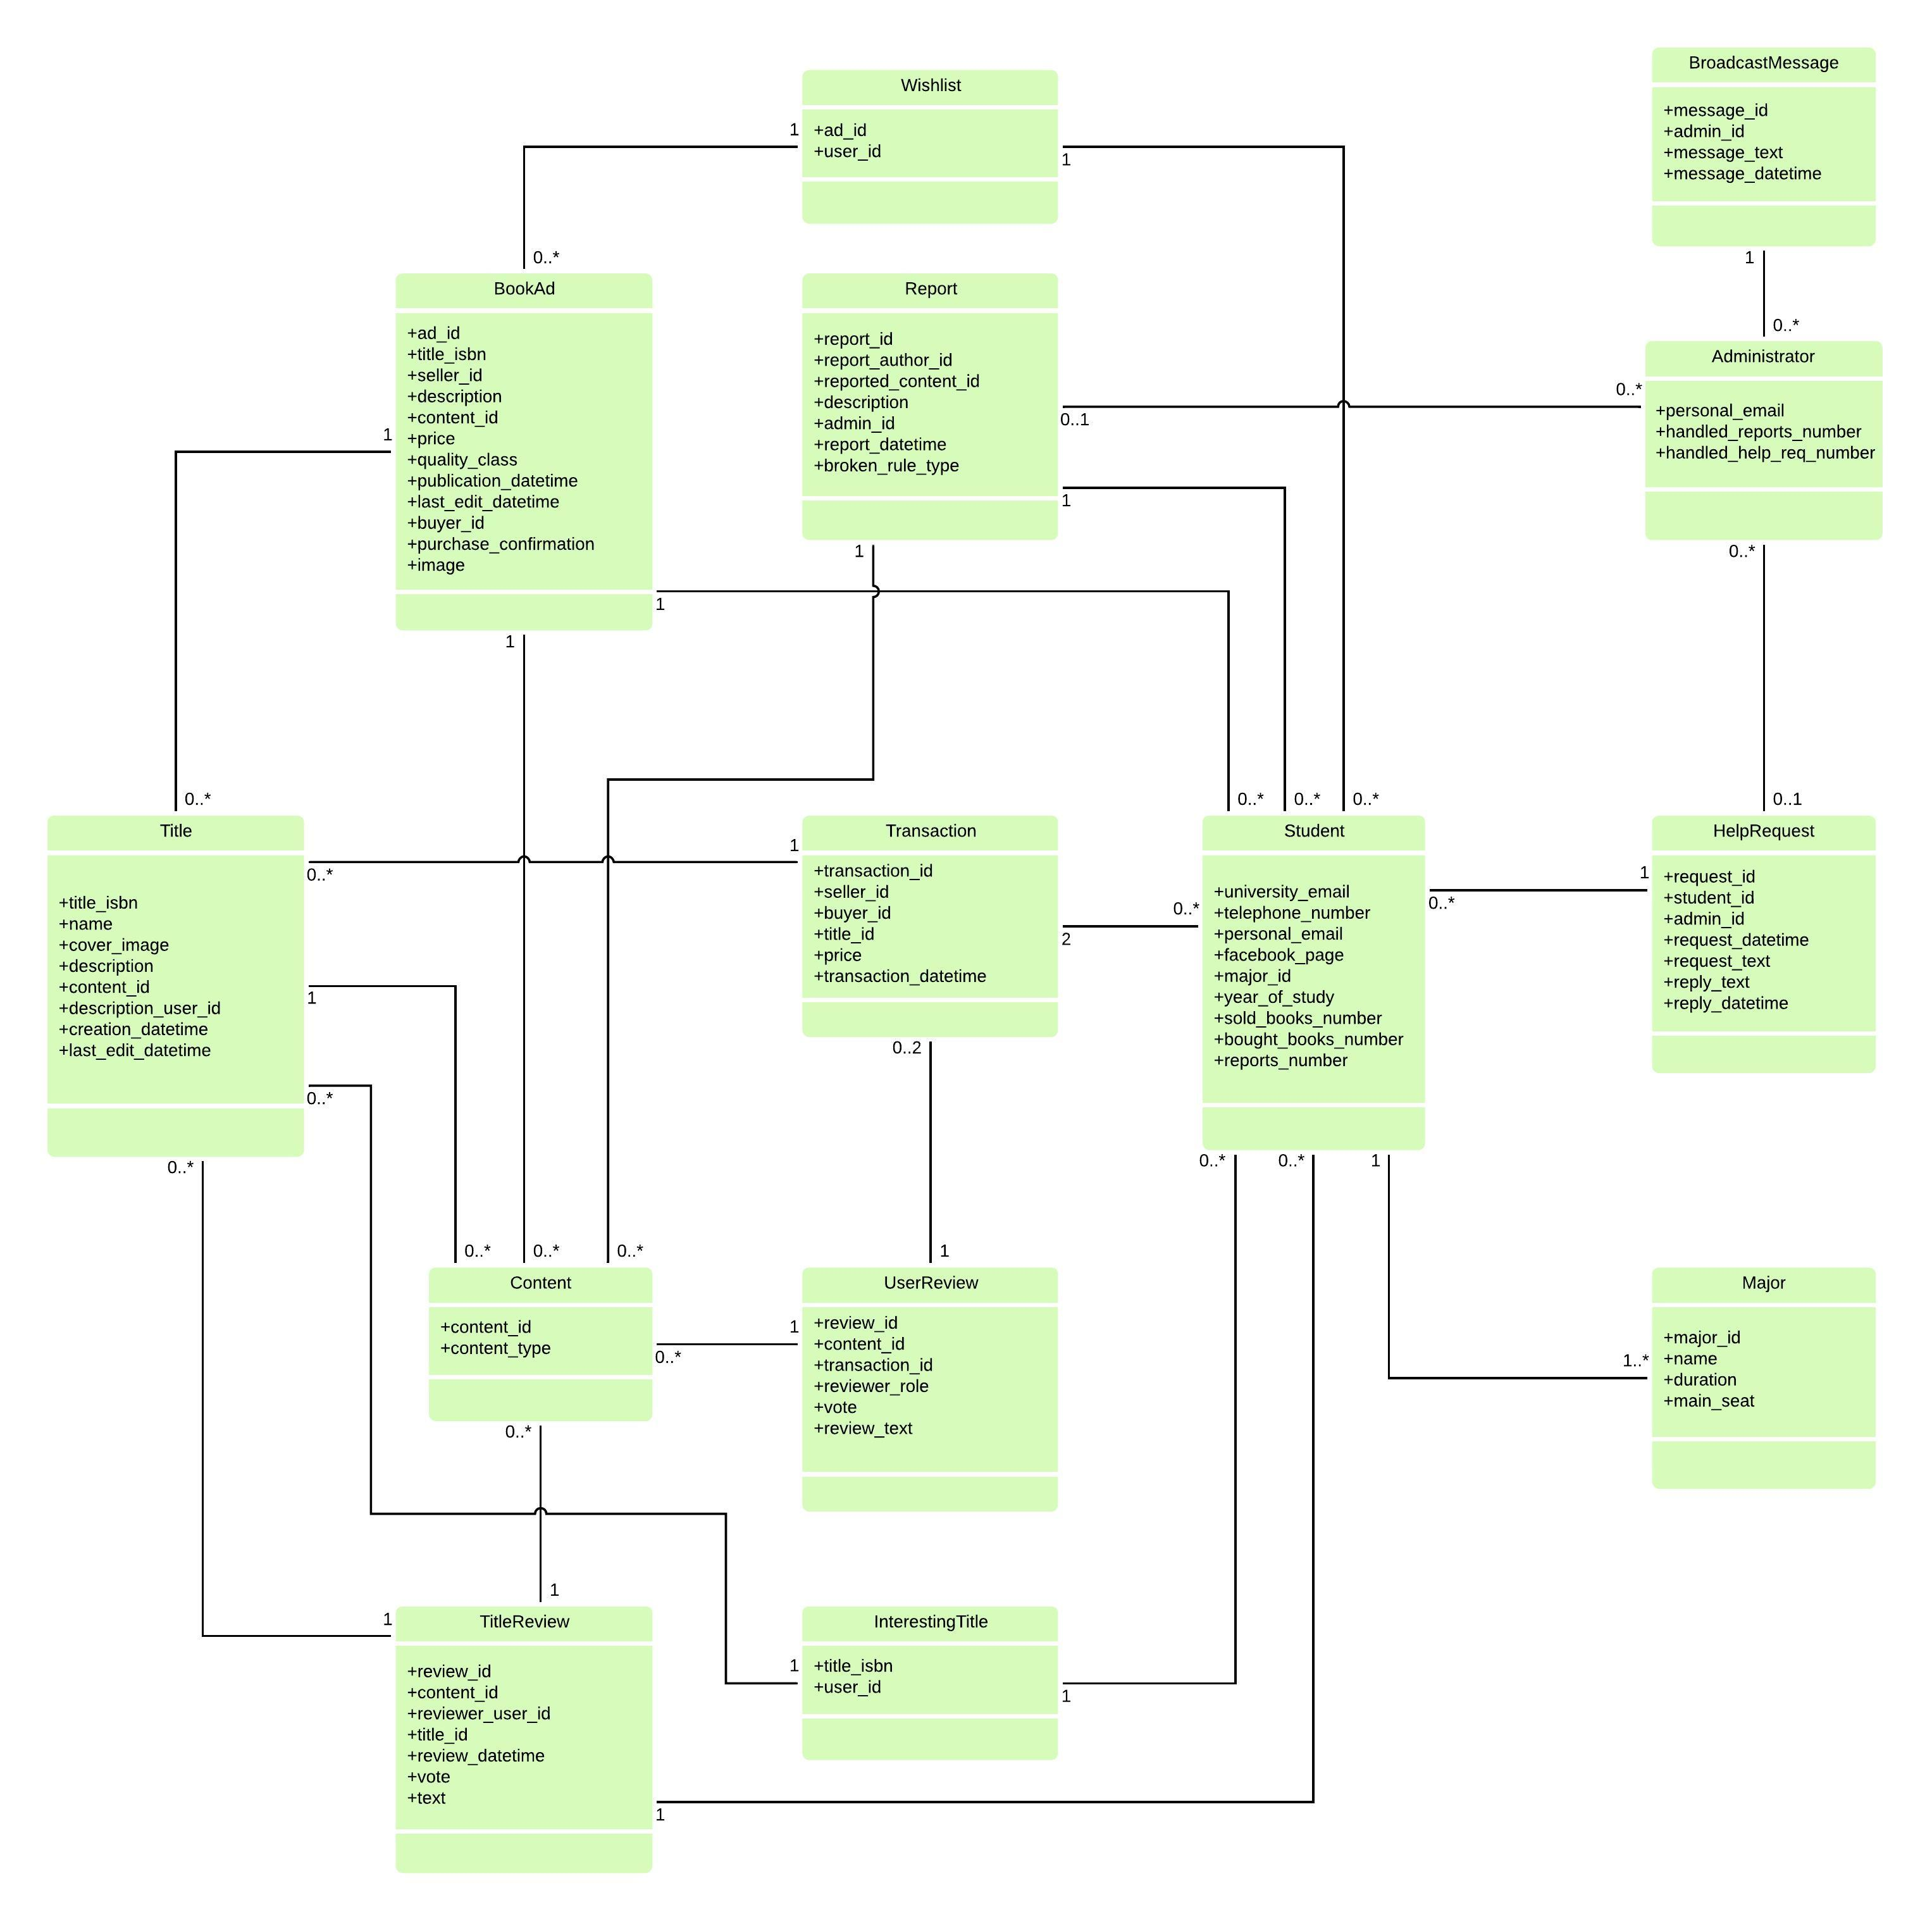
\includegraphics[height=27cm, width=17cm, keepaspectratio]{class_diagram}
		\caption{Diagramma delle classi}
	\end{figure}
	
	\section{Scelte progettuali}
	Per la realizzazione dell'applicazione sono state prese le seguenti scelte progettuali:
	\begin{itemize}
		\item Tipologia di applicazione: applicazione web, in modo da garantire un accesso semplice da qualsiasi tipo di dispositivo.
		\item Linguaggio di programmazione per l'applicazione back-end: Python 3 - framework Django 2.1, framework moderno che offre numerosi servizi di default, linguaggio ordinato e di facile lettura.
		\item Front-end: framework Bootstrap 4, per garantire una visualizzazione ottimale su dispositivi di dimensioni diverse.
		\item DBMS: PostgreSQL, indicato come particolarmente adatto per applicazioni che richiedono l'utilizzo di algoritmi di ricerca fuzzy. N.B. L'implementazione reale del progetto utilizzerà SQLite, in quanto le funzionalità che verranno realmente implementate non richiedono DBMS particolari.
		\item L'applicazione lavorerà in uno spazio messo a disposizione gratuitamente dal PaaS PythonAnywhere, specializzato nell'esecuzione di applicazioni Python.
	\end{itemize}

	\section{Toolchain}
	Le fasi di progettazione e codifica dell'applicazione verranno eseguite con l'ausilio dei seguenti tool:
	\begin{itemize}
		\item TexStudio: realizzazione della documentazione.
		\item LucidChart: realizzazione di schemi in linguaggio UML.
		\item PyCharm: IDE specifico per la programmazione in Python.
		\item Github: versioning dell'applicazione.
	\end{itemize}
	

		
     
        
\end{document}